\chapter{要点知识}
本章是对前一章的一个补充,多数内容是初次学习群环域所非必要的内容,但对掌握Galois理论和深入学习抽象代数又不可或缺.
\section{对称群}
\begin{definition}\index{xunhuan@轮换 (cycle)}\index{duihuan@对换 (transposition)}
	设 $a_1, \ldots, a_m$ 是 $X$ 中相异的元素. 对称群 $\mathfrak{S}_X$(见\ref{eg:symmetric-group}) 中的 $m$-\textbf{轮换}$(a_1 \cdots a_m)$ 是下述映射 $\sigma: X \to X$
	\begin{gather*}
		\sigma(a_i) = a_{i+1}, \quad i \in \mathbb{Z}/m\mathbb{Z}, \\
		\sigma(x)=x, \quad x \notin \{a_1, \ldots, a_m\},
	\end{gather*}
	在此将下标 $\{1, \ldots, m\}$ 方便地视为 $\mathbb{Z}/m\mathbb{Z}$ 中元素, 即模 $m$ 的同余类. 称 $m$ 为该轮换的长度; $2$-轮换 $(a b)$ 又称\textbf{对换}. 我们称 $\mathfrak{S}_X$ 中两个轮换 $(a_1 \cdots a_m),(b_1 \cdots b_k)$ 不交, 如果 $\{a_1, \ldots, a_m\} \cap \{b_1, \ldots, b_k\} = \varnothing$. 
\end{definition}

由先前讨论可知不交的轮换对乘法相交换. 同样显然的是 $\ord\ (a_1 \cdots a_m) = m$.

\begin{proposition}[轮换分解]\label{prop:cyclic-decomposition}
	每个 $\sigma \in \mathfrak{S}_X$ 都能表成不交的轮换之积
	\[ \sigma = (a_1 a_2 \cdots) (b_1 b_2 \cdots) \cdots \]
	其中的轮换 $(a_1 \cdots),(b_1 \cdots)$ 在至多差一个顺序的意义下唯一. 由于 $1$-轮换是单位元, 乘积中可以省去.
\end{proposition}

这无非是 $X$ 在 $\sigma$ 生成的有限轮换群 $\langle\sigma\rangle$ 下的轨道分解 (引理 \ref{prop:orbit-decomp}), 每个轮换对应到一个轨道, 描述了 $\sigma$ 在该轨道上的作用.

我们称轮换分解中出现的轮换长度 $n_1, n_2, \ldots$ (包括长度为一的轮换) 为 $\sigma$ 的\textbf{轮换型}, 计重数不计顺序. 为了得到唯一性, 不妨排成 $n_1 \geq n_2 \geq \cdots$, 轮换型因之对应于整数 $n \coloneqq |X|$ 的\textbf{分拆}: $n = n_1 + n_2 + \cdots$. 上面对阶数的讨论蕴涵 $\sigma$ 的阶数等于 $n_1, n_2, \ldots$ 的最小公倍数. \index{fenchai@分拆 (partition)}
\begin{corollary}[对换分解]\label{prop:S_n-generation}
	每个 $\sigma \in \mathfrak{S}_n$ 都能表成若干对换的积,但不唯一.且群 $\mathfrak{S}_n$ 由对换 $(1i)$或$(i-1\ i)$生成, 这里 $1 < i \leqslant n$.
\end{corollary}

我们既可以将$m$-轮换拆分成$m-1$个对换之积,也可以直接通过排序算法(如冒泡排序)将其拆分,行列式中的逆序数可看为选择排序.由于对换分解不唯一,且两两不可交换,故不如轮换分解方便.

据此, 共轭作用(见\ref{def:conj-action})在对称群情形下有干净的陈述.
\begin{lemma}\label{prop:cycle-type}
	设 $\tau = (a_1 a_2 \cdots) (b_1 \cdots) \cdots$ 为上述的轮换分解, $\tau \in \mathfrak{S}_X$, 则
	\[ \sigma \tau \sigma^{-1} = (\sigma(a_1) \sigma(a_2) \cdots) (\sigma(b_1) \cdots) \cdots. \]
	作为推论, 元素 $\tau$ 的共轭类由其轮换型确定; $\mathfrak{S}_X$ 中的共轭类一一对应于轮换型 $n_1 \geq n_2 \geq \cdots$, 后者又一一对应于整数 $n = |X|$ 的分拆.
\end{lemma}

这无非是先给一个新序,置换后再回到旧序,等价于在新序下的置换.
\begin{lemma}
	存在唯一的群同态 $\sgn: \mathfrak{S}_n \to \{\pm 1\}$ 使得 $\sgn((a b)) = -1$.
\end{lemma}

若置换$\sigma\in\Ker(\sgn)$,则称为偶置换,否则为奇置换.虽然对换分解不唯一,但对换分解个数的奇偶性将始终保持一致(因为两个对换之积为一个3-轮换,不可能退化成一个对换),如何得到置换的奇偶性在交错代数(比如行列式)中将非常关键.

显然奇偶置换个数相同,为此我们可以构造一个映射,将每个偶置换乘上随意一个对换则为奇置换,容易验证这是一个双射.因此$|\mathfrak{A}_n| = n!/2$.
\begin{definition}\index{qun@群 (group)!单群 (simple group)}
	只有平凡正规子群的群称为\textbf{单群}.
\end{definition}
\begin{example}
	\begin{enumerate}
		\item 素数阶循环群是单群,而$p^n(n\geqslant2,p\text{为素数})$阶群有非平凡中心,故不是单群;
		
		\item $pq,p^2q(p,q\text{为素数})$阶群不是单群;
		
		\item $2m(m\text{为大于3奇数})$阶群不是单群.
	\end{enumerate}
\end{example}

\begin{theorem}[É. Galois]\label{prop:A_n-simple}
	当 $n \geq 5$ 时 $\mathfrak{A}_n$ 是单群.
\end{theorem}
\begin{proof}
	设 $H \lhd \mathfrak{A}_n$, $H \neq \{1\}$. 从以上性质可知找出一个 $3$-轮换 $\sigma \in H$ 即足. 兹断言取 $\sigma \in H - \{1\}$ 使得 $\left|\text{Fix}(\sigma)\right|$ 极大便是.
	
	如果 $\sigma$ 的轮换分解中只有对换, 那么分解中至少含两项如 $(i j) (k l)$, 其中 $\{i,j\} \cap \{k,l\} = \emptyset$. 由于 $n \geq 5$, 可取 $r \notin \{i,j,k, l\}$ 并定义
	\begin{equation}\label{eqn:tau-sigma-simple}
		\tau \coloneqq (k l r), \quad \sigma' \coloneqq [\tau, \sigma] = \tau\sigma\tau^{-1}\sigma^{-1} \in H \quad (\because H \lhd \mathfrak{A}_n).
	\end{equation}
	可直接验证 $i,j \in \text{Fix}(\sigma') - \text{Fix}(\sigma)$, $\sigma'(k) = r \neq k$, 以及
	\[ \text{Fix}(\sigma) - \{r\} = \text{Fix}(\sigma) - \{k, l, r\} = \text{Fix}(\sigma) \cap \text{Fix}(\tau) \subset \text{Fix}(\sigma'). \]
	综之 $\left|\text{Fix}(\sigma')\right| > \left|\mathrm{Fix}(\sigma)\right|$, 矛盾.
	
	设 $\sigma$ 的轮换分解中包含长度 $>2$ 的项 $(i j k \cdots)$. 假若 $\sigma = (i j k)$ 则是所求的 $3$-轮换; 否则因为 $\sigma$ 不可能是 $4$-轮换, $\sigma$ 除了 $i,j,k$ 之外还挪动至少两个相异元 $r, l$. 依然以 \eqref{eqn:tau-sigma-simple} 式定义 $\sigma' \in H$. 可以验证 $j \in \text{Fix}(\sigma')$, $\sigma'(k) = l \neq k$ 和
	\[ \text{Fix}(\sigma) = \text{Fix}(\sigma) - \{k,l,r\} = \text{Fix}(\sigma) \cap \text{Fix}(\tau) \subset \text{Fix}(\sigma'). \]
	仍得到矛盾 $\left|\text{Fix}(\sigma')\right| > \left|\mathrm{Fix}(\sigma)\right|$. 明所欲证.
\end{proof}
\begin{corollary}
	当$n\geqslant5$时,$\mathfrak{A}_n$是$\mathfrak{S}_n$的唯一非平凡正规子群.
\end{corollary}

利用以上结果和Sylow定理可知最小非阿贝尔单群的阶数是60,且必同构于$\mathfrak{A}_n$.

\section{群列}
\begin{definition}\label{def:exact-seq-group}\index{zhenghelie@正合列 (exact sequence)}
	考虑一列群同态
	\[ \cdots \xrightarrow{f_0} G_1 \xrightarrow{f_1} G_2 \xrightarrow{f_2} \cdots \xrightarrow{f_i} G_{i+1} \to \cdots, \]
	长度或有限或无限. 若对所有 $i$ 都有
	\[ \Image(f_i) = \Ker(f_{i+1}), \]
	则称此列\textbf{正合}. 
	\begin{figure}[htp]
		\centering
		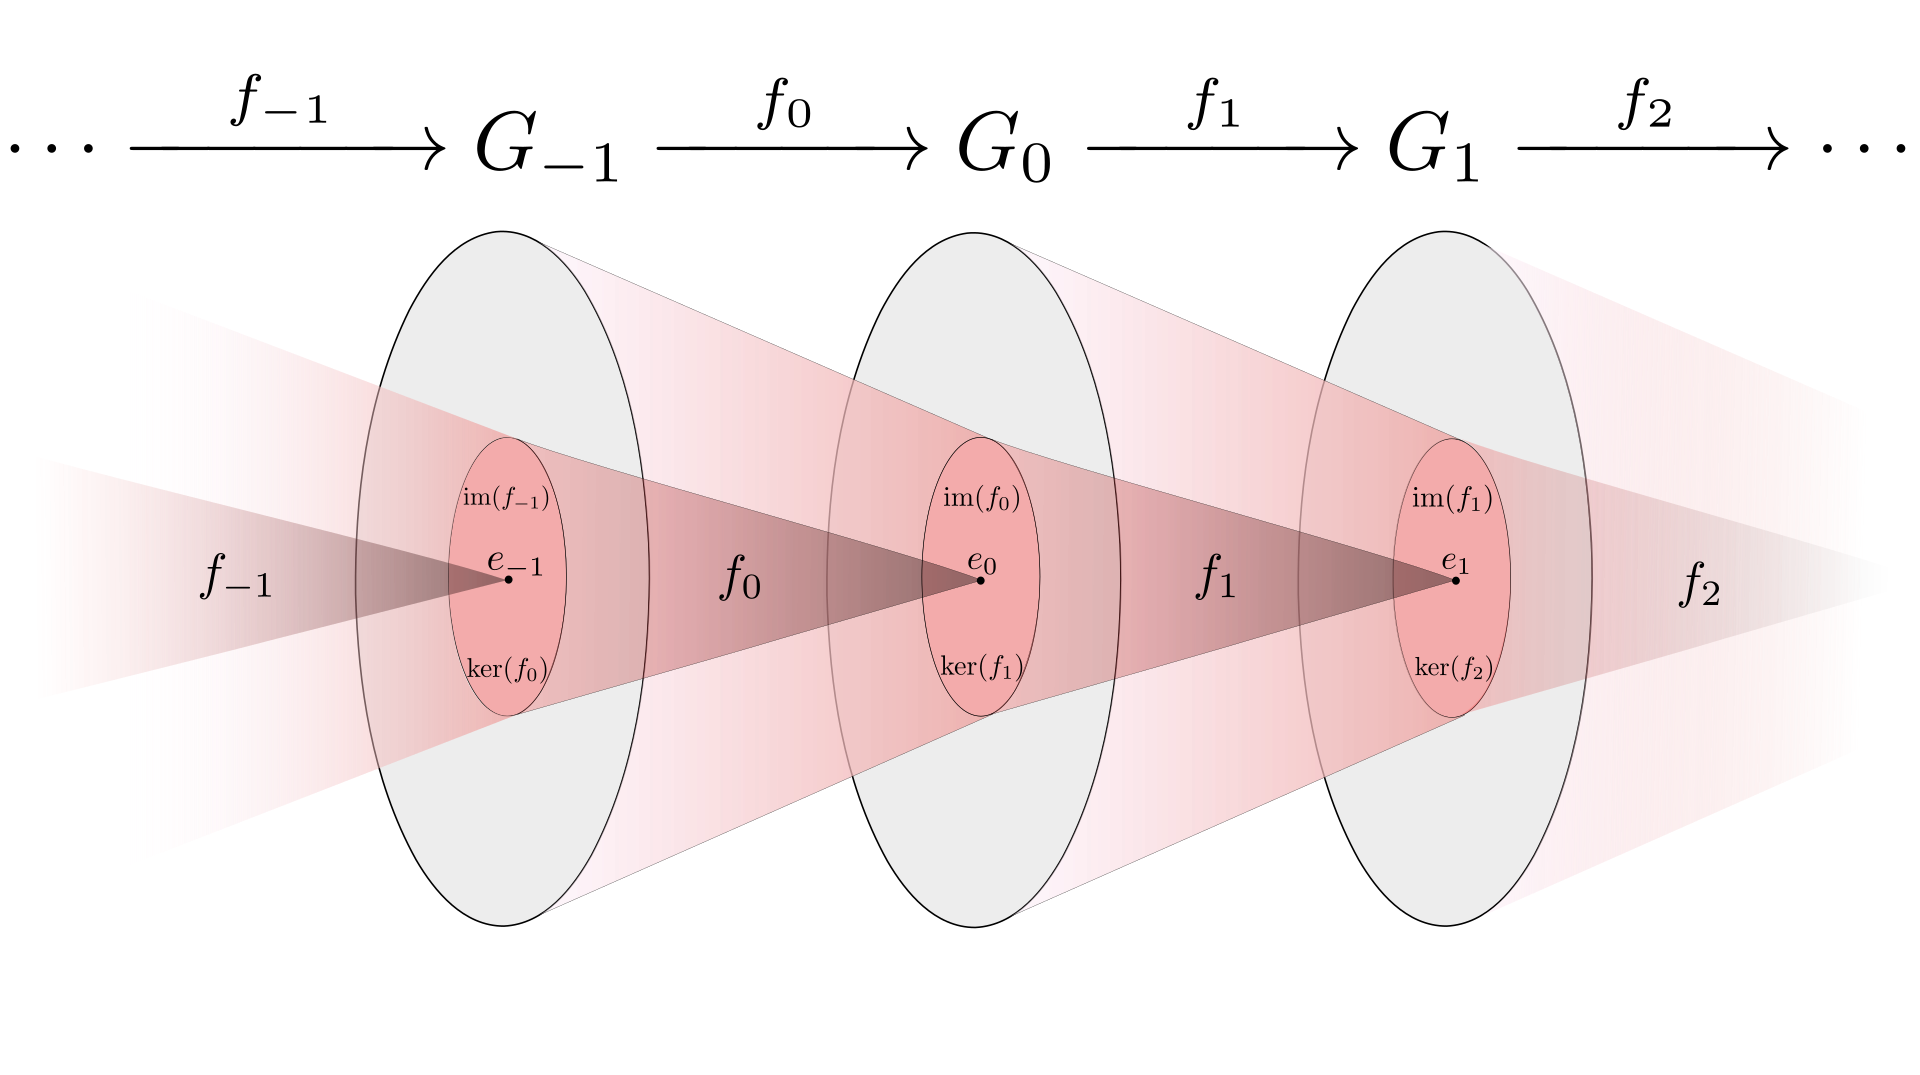
\includegraphics[scale=0.15]{Exact_Sequence_of_Groups}
		\caption{Illustration of an exact sequence of groups $G_{i}$ using Venn diagrams}
	\end{figure}
	我们经常把 $\{1\}$ 简写为 $1$, 或用加性符号记为 $0$. 举例明之, 对于任意同态 $\varphi: G \to G'$, 列 $G \to G' \to 1$ 正合当且仅当 $\varphi$ 是满的, 列 $1 \to G \to G'$ 正合当且仅当 $\varphi$ 是单的.\textbf{短正合列}为具有下列形式的正合列
	\[ 1 \to G' \xrightarrow{f} G \xrightarrow{g} G''  \to 1 \]
	如上所述,对任何一个短正合序列,$f$ 一定为单射,且$g$ 一定为满射,且$f$的像会等于$g$的核.有时也称$G$为$G''$经由$G'$的\textbf{扩张},亦即$G$可表为$G'\rtimes G''$.而若$G$可表为$G'\times G''$,则称为\textbf{平凡扩张};若$G'$落在$G$的中心,则称为\textbf{中心扩张}.
\end{definition}

正合列经常和交换图表搭配. 其妙用在同调代数中才会完全彰显,在Galois理论中将不会用到.
\begin{definition}\label{def:normal-series}\index{zhengguilie@正规列 (normal series)}\index{zhengguilie@正规列 (normal series)!次正规列 (subnormal series)}
	群 $G$ 的递降子群链
	\[ G = G_0 \geqslant G_1 \geqslant \cdots \geqslant G_n = \{1\} \]
	如满足 $\forall 0 \leq i < n,\;  G_{i+1} \lhd G_i$, 则称之为\textbf{次正规列},若还有$G_i \lhd G$则称为\textbf{正规列},而群族
	\[ G_i/G_{i+1}, \quad i=0, \ldots, n-1 \]
	称为该列的\textbf{因子群}. 正规列的\textbf{加细}是透过形如 \index{yinziqun@因子群 (factor subgroup)}
	\[ \left[ \cdots \rhd G_i \rhd G_{i+1} \rhd \cdots \right] \leadsto \left[ \cdots \rhd G_i \rhd G' \rhd G_{i+1} \rhd \cdots \right] \]
	的反复插项得到的新列. 插入 $G' = G_i$ 或 $G_{i+1}$ 得到的加细是平凡的; 反之则称为\textbf{真加细}.
\end{definition}
\begin{definition}\label{def:central-series}\index{zhongxinlie@中心列 (central series)}
	群 $G$ 的正规列 $G = G_0 \rhd G_1 \rhd \cdots$ 如对每个 $i$ 都满足
	\[
	G_i/G_{i+1} \leqslant Z_{G/G_{i+1}},
	\]
	则称为\textbf{中心列}.
\end{definition}
\begin{definition}\label{def:composition-series}\index{hechenglie@合成列 (composition series)}\index{zhuxulie@主序列 (chief series)}
	若群 $G$ 的次正规列 $G = G_0 \rhd G_1 \rhd \cdots$ 满足 $G_{i+1} \subsetneq G_i$, 而且因子群皆为单群, 则称之为\textbf{合成列},若同时为正规列,则称为\textbf{主序列}.
\end{definition}

细观单群定义可见合成列正是无冗余项, 而且无法再(真)加细的列. 有限群总有合成列, 一般的群则未必.
\begin{lemma}[Zassenhaus 蝴蝶引理]\label{prop:Zassenhaus}
	固定群 $G$, 考虑子群 $U, V$ 及各自的正规子群 $u \lhd U$, $v \lhd V$. 则有
	\begin{gather*}
		u(U \cap v) \lhd u(U \cap V), \\
		(u \cap V) v \lhd (U \cap V)v,
	\end{gather*}
	其中各项在注记 \ref{rem:HN} 的意义下都是子群, 而且有自然的同构
	\[ \dfrac{u (U \cap V)}{u (U \cap v)} \cong \dfrac{(U \cap V)v}{(u \cap V)v}. \]
\end{lemma}
\begin{proof}
	我们将表解各子群之间的关系, 图例如下:
	\[ \begin{tikzcd}
		G \arrow[dash, d] \\ H: \text{子群}
	\end{tikzcd} \quad
	\begin{tikzcd}
		G \arrow[dash, d, "\triangledown" description] \\ N: \text{正规子群}
	\end{tikzcd} \quad
	\begin{tikzcd}[column sep=tiny]
		A \arrow[dash, rd] & & B \arrow[dash, ld] \\
		& A \cap B &
	\end{tikzcd} \quad
	\begin{tikzcd}[column sep=tiny]
		{}& HN \arrow[dash, ld] \arrow[dash, rd, "\triangleleft" description] & \\
		H & & N
	\end{tikzcd}\]
	其中 $H \subset N_G(N)$. 现断言有以下图表:
	\[ \begin{tikzcd}[column sep=tiny]
		{} & U \arrow[dash, d] & & V \arrow[dash, d] & \\
		& u(U \cap V) \arrow[dash, dd, "\triangledown" description] \arrow[dash, rd] & & (U \cap V)v \arrow[dash, dd, "\triangledown" description] \arrow[dash, ld] & \\
		& & U \cap V \arrow[dash, dd, "\triangledown" description] & & \\
		& u(U \cap v) \arrow[dash, ld] \arrow[dash, rd] & & (u \cap V)v \arrow[dash, ld] \arrow[dash, rd] & \\
		u \arrow[dash, rd] & & (u \cap V)(U \cap v) \arrow[dash, ld] \arrow[dash, rd] & & v \arrow[dash, ld] \\
		& u \cap V & & U \cap v &
	\end{tikzcd} \]
	即证.故该引理也被称为蝴蝶引理.
\end{proof}
\begin{definition}\label{def:JH-subquotients}
	设 $G = G_0 \rhd \cdots$ 为次正规列, 我们视其因子群 $(G_i/G_{i+1})_{i \geq 0}$ 为不计顺序, 但计入重数的集合. 如果两个次正规列长度相同, 而且其因子群在上述意义下相等, 则称两次正规列\textbf{等价}.
\end{definition}

\begin{theorem}[Schreier 加细定理]\label{prop:Schreier}
	设
	\begin{align*}
		G & = G_0 \rhd \cdots \rhd G_r \rhd G_{r+1} = \{1\}, \\
		G & = H_0 \rhd \cdots \rhd H_s \rhd H_{s+1} = \{1\}
	\end{align*}
	为 $G$ 的两个次正规列, 则两者有等价的加细.
\end{theorem}
\begin{proof}
	对每个 $0 \leq i \leq r$, $0 \leq j \leq s$ 定义
	\begin{align*}
		G_{i,j} & \coloneqq G_{i+1} (H_j \cap G_i), \\
		H_{j,i} & \coloneqq (G_i \cap H_j) H_{j+1}.
	\end{align*}
	先看 $G_{i,j}$, 由 $G_{i+1} \lhd G_i$ 知其为子群. 包含关系 $G_{i, j+1} \lhd G_{i,j}$ 成立, 而且
	\[ G_{i,0} = G_{i+1} (G \cap G_i) = G_i, \quad G_{i,s+1} = G_{i+1}, \]
	遂得到 $(G_i)_{i=0}^r$ 的加细
	\[ \mathcal{G} \coloneqq \left[ \cdots \rhd G_i = G_{i, 0} \rhd G_{i, 1} \rhd \cdots G_{i, s} \rhd G_{i, s+1}= G_{i+1} \rhd \cdots \right] . \]
	同理可见 $H_{j, i}$ 给出 $(H_j)_{j=0}^s$ 的加细, 记为 $\mathcal{H}$. 在引理 \ref{prop:Zassenhaus} 中取 $u \coloneqq G_{i+1}$, $U \coloneqq G_i$ 和 $v \coloneqq H_{j+1}$, $V \coloneqq H_j$, 遂导出
	\[ \dfrac{G_{i,j}}{G_{i,j+1}} = \dfrac{u(U \cap V)}{u(U \cap v)} \cong \dfrac{(U \cap V)v}{(u \cap V)v} = \dfrac{H_{j,i}}{H_{j,i+1}}. \]
	
	当 $(i,j)$ 取遍所有可能, 次正规列 $\mathcal{G}$, $\mathcal{H}$ 的各个因子群在同构两边都恰好出现一次. 证毕.
\end{proof}

\begin{corollary}[Jordan--Hölder 定理]\label{cor:JH-group}
	群 $G$ 的任两个合成列皆等价.
\end{corollary}

因此, 一旦群 $G$ 有合成列, 则其因子群在定义 \ref{def:JH-subquotients} 的意义下无关合成列的选取.

\begin{definition}\index{daochulie@导出列 (derived series)}\index{zhongxinlie@中心列 (central series)!降中心列 (lower central series)}\index{zhongxinlie@中心列 (central series)!升中心列 (upper central series)}
	对于 $x, y \in G$, 定义\textbf{换位子}
	\[ [x,y] \coloneqq xyx^{-1}y^{-1}. \]
	对任意子集 $A, B \subset G$, 置 $[A, B] \lhd G$ 为 $\{[a,b] : a \in A, b \in B\}$ 的正规闭包.递归地定义
	\begin{enumerate}
		\item \textbf{导出列}: $G^{(0)} \coloneqq G, G^{(i)} \coloneqq [G^{(i-1)}, G^{(i-1)}](\forall i\geqslant1)$;
		\item \textbf{降中心列}: $G_1 \coloneqq G, G_i \coloneqq [G, G_{i-1}](\forall i\geqslant2)$;
		\item \textbf{升中心列}: $Z_0 \coloneqq \{1\},Z_{i} \coloneqq \{x\in G \mid \forall y\in G:[x,y] \in Z_{i-1} \}(\forall i\geqslant1)$.
	\end{enumerate}
\end{definition}
容易验证以下性质. 设 $i \in \mathbb{Z}_{\geq 0}$:
\begin{enumerate}
	\item $xy=yx \iff [x,y]=1$, 而 $[x,y]^{-1} = [y,x]$;
	\item 对于任意群同态 $\varphi: G_1 \to G_2$, 有 $\varphi [x,y] = [\varphi(x), \varphi(y)]$;
	\item $G^{(i)} \leqslant G_i$;
	\item $G^{(i)} \lhd G$, $G_i \lhd G$: 事实上 $G$ 的任何自同构都保持子群 $G^{(i)}$ 和 $G_i$.
	\item $G_i/G_{i+1} = Z_{G/G_{i+1}}$, $Z_i/Z_{i+1} = Z_{Z/Z_{i+1}}$.
\end{enumerate}

关于 $G^{(i)}$ 和 $G_i$ 的性质可以递归地证明. 我们也称 $G^{(1)}$ 为 $G$ 的\textbf{导出子群}或\textbf{换位子群}. 若$N\lhd G$,且$G/N$为阿贝尔群,则$G^{(1)}\leqslant N$,故 $G^\text{ab} \coloneqq G/G^{(1)}$ 称为 $G$ 的\textbf{交换化},$G$是阿贝尔群当且仅当$G^{(1)}=\{1\}$.\index{qun@群 (group)!子群 (subgroup)!导出子群 (derived subgroup)}

\begin{example}
	群 $\mathfrak{S}_n$ 的导出子群$\mathfrak{S}_n^{(1)}$ 等于 $\mathfrak{A}_n$. 当 $n \geqslant 5$ 时 $\mathfrak{A}_n$ 是非交换单群, 因此它必然等于自身的导出子群 $\mathfrak{A}_n^{(1)}$.
	
	当 $n=1$ 时此为显然. 以下解释 $n \geq 2$ 情形: $\mathfrak{S}_n$ 由对换生成, 每个对换都共轭于 $(1 \; 2)$, 故交换商 $\mathfrak{S}_n / \mathfrak{S}_n^{(1)}$ 由 $(1 \; 2)$ 的像生成, 这是二阶元. 给出商同态
	\[ \mathfrak{S}_n / \mathfrak{S}_n^{(1)} \twoheadrightarrow \mathfrak{S}_n/\mathfrak{A}_n \cong \{ \pm 1\}. \]
	比较阶数可见以上同态实为同构.
\end{example}
\section{可解群}
\begin{definition}\label{def:solvable-nilpotent-group}\index{qun@群 (group)!可解群 (solvable group)}\index{qun@群 (group)!超可解群 (supersolvable group)}\index{qun@群 (group)!幂零群 (nilpotent group)}\index{qun@群 (group)!多循环群 (polycyclic group)}
	设 $G$ 为群.给出如下等价定义:
	\begin{center}
		\begin{tabularx}{\textwidth}{cXX}
			\toprule
			&\textbf{可解群}&\textbf{幂零群}\\\midrule
			\romannumeral1)&导出列终止于$\{1\}$&降中心列终止于$\{1\}$\\
			\romannumeral2)&存在正规列使得每个因子群都交换&升中心列终止于$G$\\
			\romannumeral3)&存在次正规列使得每个因子群都交换&存在中心列\\
			\romannumeral4)&存在次正规列使得每个因子群都为素数阶循环群&存在正规列 $G = G_0 \rhd G_1 \rhd \cdots \rhd G_r = \{1\}$ 使得每个$[G,G_i]\leqslant G_{i+1}$\\
			\bottomrule
		\end{tabularx}
	\end{center}

	若存在正规列使得每个因子群都为素数阶循环群, 则称之为\textbf{超可解群};
	
	若存在次正规列使得每个因子群都为循环群, 则称之为\textbf{多循环群};
\end{definition}

设 $G$ 为幂零群, 则对任意 $x \in G$, 映射 $[x, \cdot]: g \mapsto [x, g]$ 迭代有限次次后的像落在 $\{1\}$, 故成为平凡映射 $g \mapsto 1$. 这解释了``幂零''一词的来由.而根据可解群的定义\romannumeral4),非素数阶单群是不可解的.
\begin{proposition}
	幂零蕴涵可解. 事实上,对于有限群,
	\[\text{循环群}\subset\text{阿贝尔群}\subset\text{幂零群}\subset\text{超可解群}\subset\text{多循环群}\subset\text{可解群}\subset\text{有限生成群}.\]
\end{proposition}
\begin{definition}\index{kejichengde@可继承的 (heritable)}
	性质$\mathcal{P}$称为\textbf{可继承的},若群 $G$ 具有性质 $\mathcal{P}$, 则 $G$ 的子群和商群都有性质 $\mathcal{P}$.
\end{definition}
\begin{lemma}\label{prop:solvable-ses}
	循环,阿贝尔,可解,超可解,幂零都是可继承的.
\end{lemma}

可解群的扩张亦是可解群;而幂零群的扩张未必是幂零群,但其中心扩张为幂零群.
\begin{proposition}
	设 $N \lhd G$,则 $G$ 可解当且仅当 $N,G/N$ 皆可解.
\end{proposition}

下述推论是证明五次以上方程无根式解的群论钥匙.
\begin{corollary}\label{prop:S_n-unsolvable}
	当 $n \geq 5$ 时 $\mathfrak{S}_n$ 不可解.
\end{corollary}


\begin{theorem}[Burnside $p^aq^b$定理]
	$p^aq^b$($p,q$是素数,$a,b$是正整数)阶群是可解群.
\end{theorem}

关于可解有限群最著名的结果当属英国数学家Burnside的猜想,该猜想于1963年由Walter Feit和John Griggs Thompson证明.
\begin{theorem}[Feit-Thompson 定理]\label{thm:Feit-Thompson}
	任意奇数阶有限群皆可解.
\end{theorem}

有限单群的分类是代数学里的一个巨大的工程.有关的文章大多发表于1955年至2004年之间,目的在于将所有的有限单群都给清楚地分类.这项工程总计约有100位作者在500篇期刊文章中写下了上万页的文字.该定理曾经有力地推动了有限单群的分类工作; 作为一篇有限群论的论文, 其255页的长度与繁复亦属空前, 然而还远远不是绝后的.
\begin{corollary}
	除素数阶循环群外,所有有限单群的阶都是偶数.
\end{corollary}
\section{多项式补遗}
\begin{definition}\index{huan@环 (ring)!多项式环 (polynomial ring)}\index{youlihanshuyu@有理函数域 (field of rational functions)}
	设$R$是环,$R$上以$X$为变元集的\textbf{多项式环}记作$R[X]$,包含如下元素
	\[ f = \sum_{a_1, \ldots, a_n \in \mathbb{N}\atop x_1,\dots,x_n\in X} c_{a_1, \ldots, a_n} x_1^{a_1} \cdots x_n^{a_n}. \]
	在其上有自然的加法和乘法.当$X=\{x,y,\dots\}$时,也记作$R[x,y,\dots]$.当$R$是交换环时,则称为多项式代数.设$K$是域,多项式环$F[X]$的分式域称为\textbf{有理函数域},记作$K(X)$,当$X=\{x,y,\dots\}$时,也记作$K(x,y,\dots)$.
	下标稍嫌繁杂, 我们顺势引进方便的多重指标符号,令$|X|=n$,
	\begin{align*}
		\bm{a} & \coloneqq (a_1, \ldots, a_n),\quad |\bm{a}| \coloneqq a_1 + \cdots + a_n,\quad c_{\bm{a}} \coloneqq c_{a_1, \ldots, a_n}, \\
		\bm{x}& \coloneqq(x_1,x_2,\dots,x_n),\quad \bm{x}^{\bm{a}} \coloneqq x_1^{a_1} \cdots x_n^{a_n}.\\
		&\implies f=\sum_{\bm{a}\in \mathbb{N}^n} c_{\bm{a}} \bm{x}^{\bm{a}}.
	\end{align*}
	
	注意到$R[x,y]=R[x][y]$.
\end{definition}
\begin{definition}\index{cishu@次数 (degree)}
	定义多项式 $f$ 的\textbf{次数}为 $\deg f \coloneqq \max\left\{ |\bm{a}| : |c_{\bm{a}}|\neq 0 \right\}$. 如果 $f$ 满足于 $c_{\bm{a}} \neq 0 \iff |\bm{a}|=m$, 则称 $f$ 是 $m$ 次\textbf{齐次多项式}.
\end{definition}
\begin{example}
	若$K$是域,在定义 \ref{def:Euclidean-ring} 中取$\deg$使得$K[X]$为ED.
\end{example}
\begin{example}\label{eg:Gauss-integers}
	Gauss 整数环定义为
	\[ \mathbb{Z}[\sqrt{-1}] \coloneqq \left\{ x+y\sqrt{-1} : x,y \in \mathbb{Z} \right\} \quad \text{(作为 $\mathbb{C}$ 的子环)}. \]
	在定义 \ref{def:Euclidean-ring} 中取范数映射
	\[ N(x+y\sqrt{-1}) = |x+y\sqrt{-1}|^2 = x^2 + y^2 \;\in \mathbb{N}. \]
	使得其为ED.
	
	
	注意到 $\mathbb{Z}[\sqrt{-1}]$ 对共轭运算 $z \mapsto \bar{z}$ 封闭, $N(z)=z\bar{z}$ 是乘法幺半群的同态, 由此不难推得 $\mathbb{Z}[\sqrt{-1}]^\times = N^{-1}(\mathbb{Z}^\times) = \{\pm 1, \pm\sqrt{-1}\}$.
\end{example}
\begin{proposition}
	若$R$是UFD/整环,则$R[X]$亦然.域上的一元多项式环为PID;环上则未必,如$\mathbb{Z}[\sqrt{5}].$
\end{proposition}
\begin{definition}\index{huan@环 (ring)!Noether环 (Noetherian ring)}
	称环$R$为\textbf{Noether环},若$R$的任一理想都是有限生成的.
\end{definition}
\begin{theorem}[Hilbert基定理]
	若$R$为Noether环,则$R[x]$亦然.
\end{theorem}

该定理与\textbf{Hilbert零点定理(Nullstellensatz)}相关,后者是代数几何中的基本定理.
\begin{definition}\index{duichengduoxiangshi@对称多项式 (symmetric polynomial)}
	称一个多项式$f\in R[X]$为\textbf{对称多项式},若$\forall \sigma\in \mathfrak{S}_X$, $f(\bm{x})=f(\sigma\bm{x})$.记所有的$n$元对称多项式构成的环为$\Lambda_n$.
\end{definition}
\begin{definition}\index{duichengduoxiangshi@对称多项式 (symmetric polynomial)!初等对称多项式 (elementary symmetric polynomial)}\label{def:ele-sym}
	定义$\bm{x}$的第$k$个$n$元\textbf{初等对称多项式}为
	\[e_k\coloneqq\sum_{1 \leq i_1 < \cdots < i_k \leq n} x_{i_1} \cdots x_{i_n}.\]
\end{definition}
\begin{theorem}[对称多项式基本定理]\label{thm:sym-basic}
	设$R$是环,$f\in \Lambda_n$是$R$上的对称多项式当且仅当是一些$n$元初等对称多项式的代数组合.即$\Lambda_n\cong R[e_1,e_2,\dots,e_n]$.
\end{theorem}